%%%%%%%%%%%%%%%%%%%%%%%%%%%%%%%%%%%%%%%%%%%%%%%%%%%%%%%%%%%%%%%%%%%%%%%%%%%%%%%%%%%%%%%%%%%%%%%%
%
% CS576 Written Question Template
%
% Acknowledgements:
% The original code is written by Prof. James Tompkin (james_tompkin@brown.edu).
% The second version is revised by Prof. Min H. Kim (minhkim@kaist.ac.kr).
%
% This is a LaTeX document. LaTeX is a markup language for producing
% documents. Your task is to fill out this document, then to compile
% it into a PDF document.
%
%
% TO COMPILE:
% > pdflatex thisfile.tex
%
% If you do not have LaTeX and need a LaTeX distribution:
% - Personal laptops (all common OS): www.latex-project.org/get/
% - We recommend latex compiler miktex (https://miktex.org/) for windows,
%   macTex (http://www.tug.org/mactex/) for macOS users.
%   And TeXstudio(http://www.texstudio.org/) for latex editor.
%   You should install both compiler and editor for editing latex.
%   The another option is Overleaf (https://www.overleaf.com/) which is
%   an online latex editor.
%
% If you need help with LaTeX, please come to office hours.
% Or, there is plenty of help online:
% https://en.wikibooks.org/wiki/LaTeX
%
% Good luck!
% Min and the CS576 staff
%
%%%%%%%%%%%%%%%%%%%%%%%%%%%%%%%%%%%%%%%%%%%%%%%%%%%%%%%%%%%%%%%%%%%%%%%%%%%%%%%%%%%%%%%%%%%%%%%%
%
% How to include two graphics on the same line:
%
% \includegraphics[\width=0.49\linewidth]{yourgraphic1.png}
% \includegraphics[\width=0.49\linewidth]{yourgraphic2.png}
%
% How to include equations:
%
% \begin{equation}
% y = mx+c
% \end{equation}
%
%%%%%%%%%%%%%%%%%%%%%%%%%%%%%%%%%%%%%%%%%%%%%%%%%%%%%%%%%%%%%%%%%%%%%%%%%%%%%%%%%%%%%%%%%%%%%%%%

\documentclass[11pt]{article}

\usepackage[english]{babel}
\usepackage[utf8]{inputenc}
\usepackage[colorlinks = true,
            linkcolor = blue,
            urlcolor  = blue]{hyperref}
\usepackage[a4paper,margin=1.5in]{geometry}
\usepackage{stackengine}
\usepackage{graphicx}
\usepackage{fancyhdr}
\setlength{\headheight}{15pt}
\usepackage{microtype}
\usepackage{times}
\usepackage{booktabs}

\usepackage{listings}

\usepackage{caption} %table caption

\usepackage{courier} %package for code font

\usepackage{array} %package for tables

\usepackage[]{algorithm2e}

\usepackage{float} %Package used for images placements "[H]"


\usepackage{subcaption} %package for subplot

\renewcommand{\vec}[1]{\mathbf{#1}}

\usepackage[backend=biber]{biblatex} %Imports biblatex package
\addbibresource{references.bib} %Import the bibliography file

% From https://ctan.org/pkg/matlab-prettifier
\usepackage[numbered,framed]{matlab-prettifier}

\frenchspacing
\setlength{\parindent}{0cm} % Default is 15pt.
\setlength{\parskip}{0.3cm plus1mm minus1mm}

\pagestyle{fancy}
\fancyhf{}
\lhead{Homework 2 Writeup - Krzysztof Palczewski (20196151)}
\rhead{CS576}
\rfoot{\thepage}

\date{}

\title{\vspace{-1cm}Homework 2 Writeup}


\begin{document}
\maketitle
\vspace{-3cm}
\thispagestyle{fancy}

%\section*{Instructions}
%\begin{itemize}
%  \item Describe any interesting decisions you made to write your algorithm.
%  \item Show and discuss the results of your algorithm.
%  \item Feel free to include code snippets, images, and equations.
%  \item There is no page limit.
%
%\end{itemize}

\section*{Objective of the work}

The main goal of the work is to implement visual recognition of different environments based on feature descriptors. There are 15 labels of images and there are 100 images from each category in training, as well as test set.

\begin{figure}[H]
    \centering
    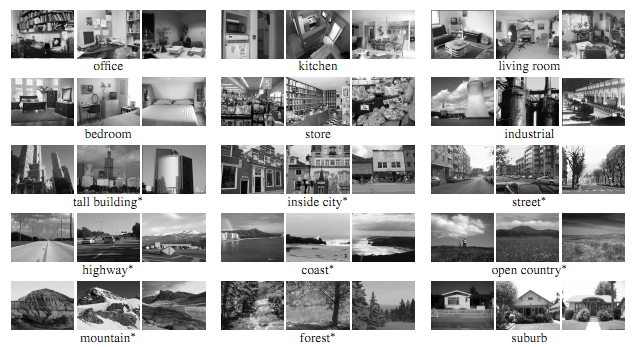
\includegraphics[width=10cm]{categories.jpg}
    \caption{Exemplary images from the dataset \cite{lazebnik2006beyond}}
    \label{fig:dataset}
\end{figure}

Process of performing visual recognition of depicted environments could be seen as a sequence of following processes:

\begin{figure}[H]
    \centering
    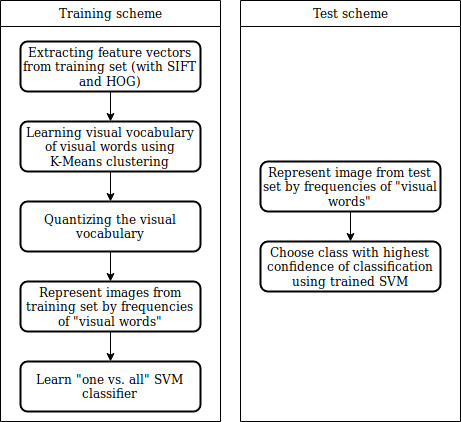
\includegraphics[width=7cm]{flow_scene_recognition.jpg}
    \caption{Flow chart of scene recognition scheme}
    \label{fig:flowchart_scene_recognition}
\end{figure}

\section*{Building vocabulary by k-means clustering}

    \subsection*{Feature extraction}
In the exercise I used two feature extractors: Histogram of oriented gradients (HOG) and Scale-invariant feature transform (SIFT) algorithm.\\
HOG algorithm breaks image to cells, compute histogram of oriented gradients in the cells, normalize output across the block formed from cells and add up all gradients. I used \texttt{cv2.HOGDescriptor()} function, which returns concatenated list for all feature, which has to be re-scaled to size $(num\_features \times 36)$.\\
SIFT algorithm uses scale-space extrema detection with gaussian kernel ans keypoint localization to find relevant features. I used \texttt{cv2.xfeatures2d.SIFT\_create()} which returns list of features of size $(num\_fatures \times 36)$. Code which performs feature extraction is shown below:

\begin{lstlisting}[language=Python]
def feature_extraction(img, feature):
    """
    This function computes defined feature (HoG, SIFT) descriptors of the target image.

    :param img: a height x width x channels matrix,
    :param feature: name of image feature representation.

    :return: a N x feature_size matrix.
    """

    if feature == 'HoG':

        win_size = (32, 32)
        block_size = (32, 32)
        block_stride = (16, 16)
        cell_size = (16, 16)

        nbins = 9
        deriv_aperture = 1
        win_sigma = 4
        histogram_norm_type = 0
        l2_hys_threshold = 2.0000000000000001e-01
        gamma_correction = 0
        nlevels = 64

        # Your code here. You should also change the return value.

        # sample visualizing
        # cv2.imshow('img', img)

        gray = cv2.cvtColor(img, cv2.COLOR_BGR2GRAY)


        hog = cv2.HOGDescriptor(win_size,
                                block_size,
                                block_stride,
                                cell_size,
                                nbins,
                                deriv_aperture,
                                win_sigma,
                                histogram_norm_type,
                                l2_hys_threshold,
                                gamma_correction,
                                nlevels)

        hist = hog.compute(gray)
        hist_resized = np.resize(hist, (int(len(hist)/36), 36))
        hist_resized
        return hist_resized

    elif feature == 'SIFT':

        gray = cv2.cvtColor(img, cv2.COLOR_BGR2GRAY)
        sift = cv2.xfeatures2d.SIFT_create()
        kp, des = sift.detectAndCompute(gray, None)

        return des

\end{lstlisting}

    \subsection*{Learning visual vocabulary using K-means clustering}
After feature extraction there are multiple features for every image. To build "viusal vocabulary" from "visual words". "Visual vocabulary" is a set of unique features derived from the training set. With the assumptions that there are regions where density of real features are higher, we could find those regions by K-means clustering.

\begin{algorithm}[H]
 \SetKwInOut{Parameter}{parameter}
 \KwData{Visual words}
 \KwResult{List of code vectors}
 \Parameter{max\_iter = 100, epsilon = 1e-4}
 Find maximum (max\_feat) and minimum value (min\_feat)\\
 of each feature \\
 Randomly assign centroids in the range \<max\_feat, min\_feat\>\\
 \While{iter $<$ max\_iter}{
  assign points to nearest centroids\;
  \For{every centroid $c$}{
    \eIf{there are any points assigned to centroid}{
        compute mean of assigned points $mean_c$;\\
        compute distance between mean of assigned points and centroid $d_c$;\\
        change position of c to mean: $c$ = $mean_c$;\\
        }
        {
        leave centroid in the same place;
        }
    \eIf{$d_c$ for every centroid $<$ $epsilon$}{
        return $c$}
  }
  return $c$
 }
 
 \caption{Building visual vocabulary with K-means}
\end{algorithm}


        \subsubsection*{Principle component analysis(PCA) for vocabulary}
Feature space for HOG algorithm equals 36 and for SIFT algorithm 128. Since it is impossible to visualize in a meaningful way such high dimensional data, we could use PCA for such task. PCA could be also perform as a preprocessing step to reduce the dimensionality of the data and to decrease the variance of our model.

\begin{figure}[H]
\begin{subfigure}{.5\textwidth}
  \centering
  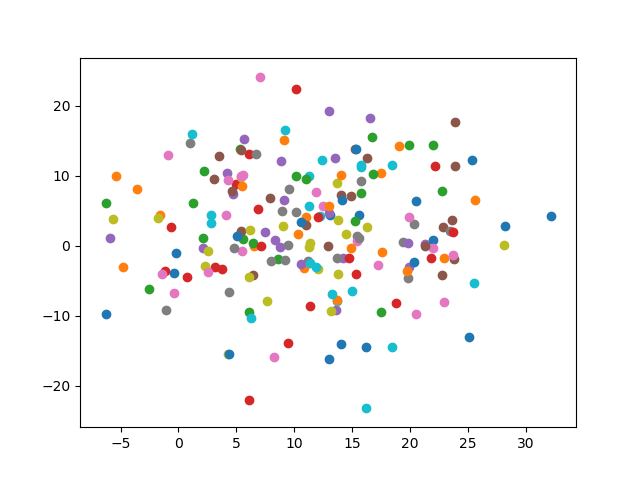
\includegraphics[width=.8\linewidth]{PCA_sift_2d.png}
  \caption{First 2 PC for SIFT algorithm}
  \label{fig:PCA_sift_2d}
\end{subfigure}%
\begin{subfigure}{.5\textwidth}
  \centering
  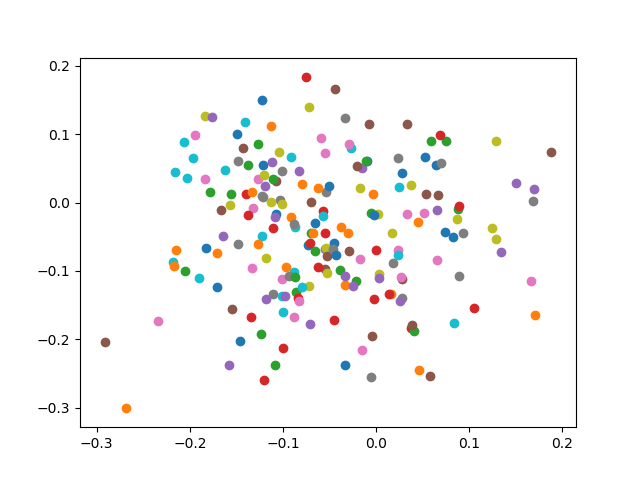
\includegraphics[width=.8\linewidth]{PCA_HOG_2d.png}
  \caption{First 2 PC for HOG algorithm}
  \label{fig:PCA_hog_2d}
\end{subfigure}
\caption{First 2 Principal Components for SIFT and HOG algorithm}
\label{fig:PCA_2d}

\begin{subfigure}{.5\textwidth}
  \centering
  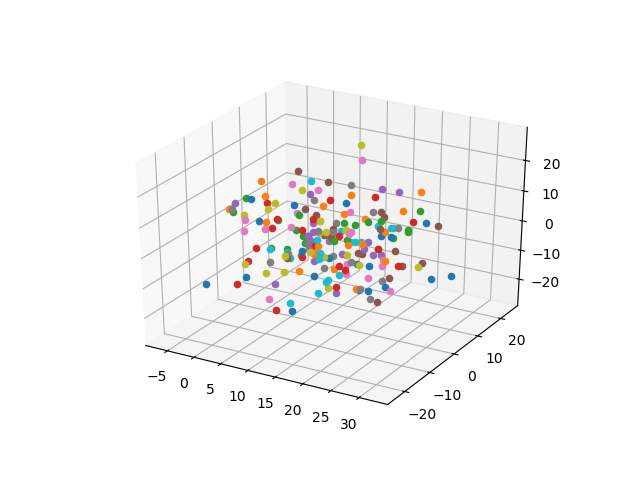
\includegraphics[width=.8\linewidth]{PCA_sift_3d.png}
  \caption{First 3 PC for SIFT algorithm}
  \label{fig:PCA_sift_3d}
\end{subfigure}%
\begin{subfigure}{.5\textwidth}
  \centering
  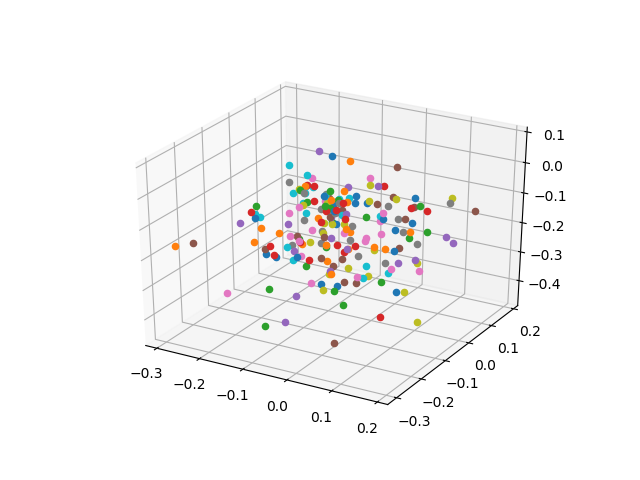
\includegraphics[width=.8\linewidth]{PCA_HOG_3d.png}
  \caption{First 3 PC for HOG algorithm}
  \label{fig:PCA_hog_3d}
\end{subfigure}
\caption{First 3 Principal Components for SIFT and HOG algorithm}
\label{fig:PCA_3d}
\end{figure}

Function which performs PC extraction is shown below:
\begin{lstlisting}[language=Python]
def get_features_from_pca(feat_num, feature):
    """
    This function loads 'vocab_sift.npy' or 'vocab_hog.npg' file and
    returns dimension-reduced vocab into 2D or 3D.

    :param feat_num: 2 when we want 2D plot, 3 when we want 3D plot
    :param feature: 'Hog' or 'SIFT'

    :return: an N x feat_num matrix
    """

    if feature == 'HoG':
        vocab = np.load('vocab_hog.npy')
    elif feature == 'SIFT':
        vocab = np.load('vocab_sift.npy')

    def _get_PCA_vectors(feat_num, vocab):

        mean = vocab.mean(axis=0, keepdims=True)
        vocab_normalized = vocab - np.multiply(np.ones([vocab.shape[0], 
            mean.shape[0]]), mean)
        #TEST: mean unit test
        #mean = vocab_normalized.mean(axis=0, keepdims=True)

        cov_matrix = np.cov(np.transpose(vocab_normalized))
        sigma, V = np.linalg.eig(cov_matrix)
        order_sigma = np.argsort(sigma)

        PCA_vectors = []
        i = 1
        for f in range(len(order_sigma)):
            eigen_vector = V[:, order_sigma[i]]
            if all(True for _ in np.isreal(eigen_vector)):
                PCA_vectors.append(np.real(eigen_vector))
                i += 1
            if len(PCA_vectors) == feat_num:
                break

        return np.array(PCA_vectors)

    #MAIN
    PCA_vectors = _get_PCA_vectors(feat_num, vocab)

    d = np.dot(vocab, np.transpose(PCA_vectors))

    return np.dot(vocab, np.transpose(PCA_vectors))
\end{lstlisting}

\section*{Representing images from training set by frequencies of "visual words"}
I implemented 2 approaches (Bag of words and Spatial Pyramid) to combine features obtain from every image into meaningful low-dimensional input into SVM classifier.

    \subsection*{Bag of words representation of scenes}
Bag of words implementation involve representing features of every image by code vectors of the "visual vocabulary" and combining those codevectors into normalized histogram of occurrences. Bag of words implementation doesn't contain any information about spatial location and proximity between features.

    \subsection*{Spatial pyramid representation}
Spatial pyramid representation is a more complex form than Bag of words, which involves also information about spatial location of features obtaining for every image. In this approach histogram of features is obtained by weighted sum of histograms for multiple levels of images. Each level of images involve $4^l$ equal sized subimages of the original image.

\section*{Multi-class SVM}
Having representation of images from training set by frequencies of "visual words" the next step is to learn SVM classifier which would be capable to recognize environments from \cite{lazebnik2006beyond}.
SVM classifier is a binary classifier, so to obtain the classification task between 15 classes in the model I trained 15 "one vs. all". For every image there are 15 probabilities that the class is the choosen one. In the training set for every image is chosen class which has the highest probability obtained by "one vs. all" classifier for this class. Code which executes "one vs. all" classificator is shown below:

\begin{lstlisting}[language=Python]
    categories = np.unique(train_labels)

    categories_dict = dict(zip(np.arange(15), categories))

    all_predicted_proba = np.empty([1500,1])

    for c in range(len(categories)):
        one_vs_all_labels = [1 if n == categories[c] 
            else -1 for n in train_labels]
        clf = svm.SVC(probability=True, gamma='auto', 
            kernel=kernel_type)
        clf.fit(train_image_feats, one_vs_all_labels)
        predicted_proba = clf.predict_proba(test_image_feats)
        predicted_proba = predicted_proba[:,1].
            reshape((len(predicted_proba[:,1]),1))
        all_predicted_proba = np.hstack((all_predicted_proba,
                                        predicted_proba))

    all_predicted_proba = all_predicted_proba[:,1:]

    max_proba = np.argmax(all_predicted_proba, axis=1)

    out_labels = np.array([categories_dict[x] 
        for x in max_proba])

    return out_labels
\end{lstlisting}

    \subsection*{The kernel trick}
SVM classification could be obtain by solving Dual problem:
$$ max L_{D}(a_{i}) = \Sigma^{l}_{i=1} - \frac{1}{2}\Sigma^{l}_{i=1}a_{i}a_{j}y_{i}y_{j}(\vec{x_{i}}\cdot\vec{x_{j}})s.t.$$
$\Sigma^{l}_{i=1}a_{i}y_{i} = 0$ \& $a_{i} >= 0 $
We obtain coefficients $a$ by nonlinear optimization and in the training process to obtain the classification we only have to compute $(\vec{x_{i}}\cdot\vec{x_{j}})$, between all training examples for which $a_{i}=0$ and new point ($a_{i}$ is non-zero only for support vectors). This term could be wraped into to different kernel functions $K(\vec{x_{i}}\cdot\vec{x_{j}})$ to imitate feature expansion to get non-linear SVM decision boundary.\\

We could use radial basis function (RBF) kernel, which we get by computing:
$$
K_{RBF}(\vec{x_{i}}\cdot\vec{x_{j}}) = e^{-\gamma||\vec{x_{i}} - \vec{x_{j}}||^{2}}
$$
When parameter $\gamma$ is higher we place lower impact on the difference between training points and new observation, so the "area of influence of support vectors is lower" and model is prone to overfitting.

\section*{Accuracy of the model}
    
    \subsection*{Comparsion of SIFT and HOG performance}
In the model I used two feature exctractors SIFT and HOG.

\begin{tabular}{ |p{3cm}|p{3cm}|p{3cm}|p{3cm}|  }
 \hline
 Feature extractor & Kernel & Representation & Accuracy\\
 \hline \hline
 SIFT & Linear & Bag of words & $43.0 \%$\\ \hline
 HOG & Linear & Bag of words & $41.9\%$\\ \hline \hline
 SIFT & Linear & Spatial pyramid & $46.4\%$\\ \hline \hline
 HOG & Linear & Spatial pyramid & $46.3\%$\\ \hline
\end{tabular}
\captionof{table}{Comparsion of overall accuracy of the model between SIFT and HOG}
    
As shown in table 1 SIFT features has $1.1\%$ higher accuracy on the used dataset than HOG using Bag of words and $0.1\%$ higher with use Spatial pyramid. The reason could be fact that, as mentioned above SIFT features include information about spatial location of the feature. Though, in the model especially with use of Spatial pyramid increase in the accuracy is not siginificant and depending on the task Bag of words could be better choice since computational complexity for this algorithm is significantly lower than for Spatial Pyramid.

    \subsection*{Comparsion of linear and RBF kernel}
In the model I used linear and RBF kernels SVM classifier.\\
    
\begin{tabular}{ |p{3cm}||p{3cm}|p{3cm}|p{3cm}|  }

 \hline
 Feature extractor & Kernel & Representation & Accuracy\\
 \hline \hline
 SIFT   & Linear & Bag of words & 43.0\%\\ \hline
 SIFT   & RBF & Bag of words & 17.7\%\\ \hline \hline
 HOG &   Linear  & Bag of words & 41.9\%\\ \hline
 HOG &   RBF  & Bag of words & 23.2\%\\ \hline \hline
 SIFT   & Linear & Spatial pyramid & 46.4\%\\ \hline
 SIFT   & RBF & Spatial pyramid & 46.2\%\\ \hline \hline
 HOG &   Linear  & Spatial pyramid & 46.3\%\\ \hline
 HOG &   RBF  & Spatial pyramid & 46.7\%\\ 
 \hline
\end{tabular}
\captionof{table}{Comparsion of overall accuracy of the model between Linear and RBF kernel}

\hfill \break 
Table 2 shows the comparsion between RBF and linear kernels. For the RBF kernel I used $\gamma$ in the 'auto' mode which uses value $\frac{1}{number\_of\_features}$. Radial kernel has much higher variance than linear kernel and SVM classifier is much more unstable than in case of linear kernel. One could see it for the Bag of words approach, when for dafault values of $\gamma$ mode has $23.3\%$ and $18.7\%$ lower accuracy!

With use of Bag of words RBF kernel has similar accuracy to linear kernel, with the best accuracy among all  models which is $46.7\%$

    \subsection*{Comparsion of Bag of Words and Spatial Pyramid}
In the model I used Bag of Words and Spatial Pyramid representation.

\begin{tabular}{ |p{3cm}||p{3cm}|p{3cm}|p{3cm}|  }

 \hline
 Feature extractor & Kernel & Representation & Accuracy\\
 \hline \hline
 SIFT   & Linear & Spatial pyramid & 46.4\%\\ \hline 
 SIFT   & Linear & Bag of words & 43.0\%\\ \hline \hline
 HOG &   Linear  & Spatial pyramid & 46.3\%\\ \hline 
 HOG &   Linear  & Bag of words & 41.9\%\\ \hline \hline
 SIFT   & RBF & Spatial pyramid & 46.2\%\\ \hline
 SIFT   & RBF & Bag of words & 17.7\%\\ \hline \hline
 HOG &   RBF  & Spatial pyramid & 46.7\%\\ \hline 
 HOG &   RBF  & Bag of words & 23.2\%\\ \hline
\end{tabular}
\captionof{table}{Comparsion of overall accuracy of the model between Bag of Words and Spatial Pyramid}
\hfill \break
Table 3 shows that on average Bag of Words has on average $2.4\%$ lower accuracy using linear kernel than Spatial Pyramid and $26\%$ lower using RBF kernel. It is a significant difference and in many more complex task, Spatial Pyramid could outperform Bag of Words.

\section*{Future works}
In the further development of the model one could use Cross Validation scheme to try multiple kernels, and $\gamma$ values. Also more training points could be used during the training process.

\begin{figure}[H]
    \printbibliography
\end{figure}

\end{document} 
